\appendix
\section{Dimensions of the obstacles}
As discussed in section \ref{obstacles}, the obstacles used in the CFD analysis were estimated using Google Maps. In figure \ref{maps} it is shown how these distances were estimated. 
\begin{figure}[b]
\centering
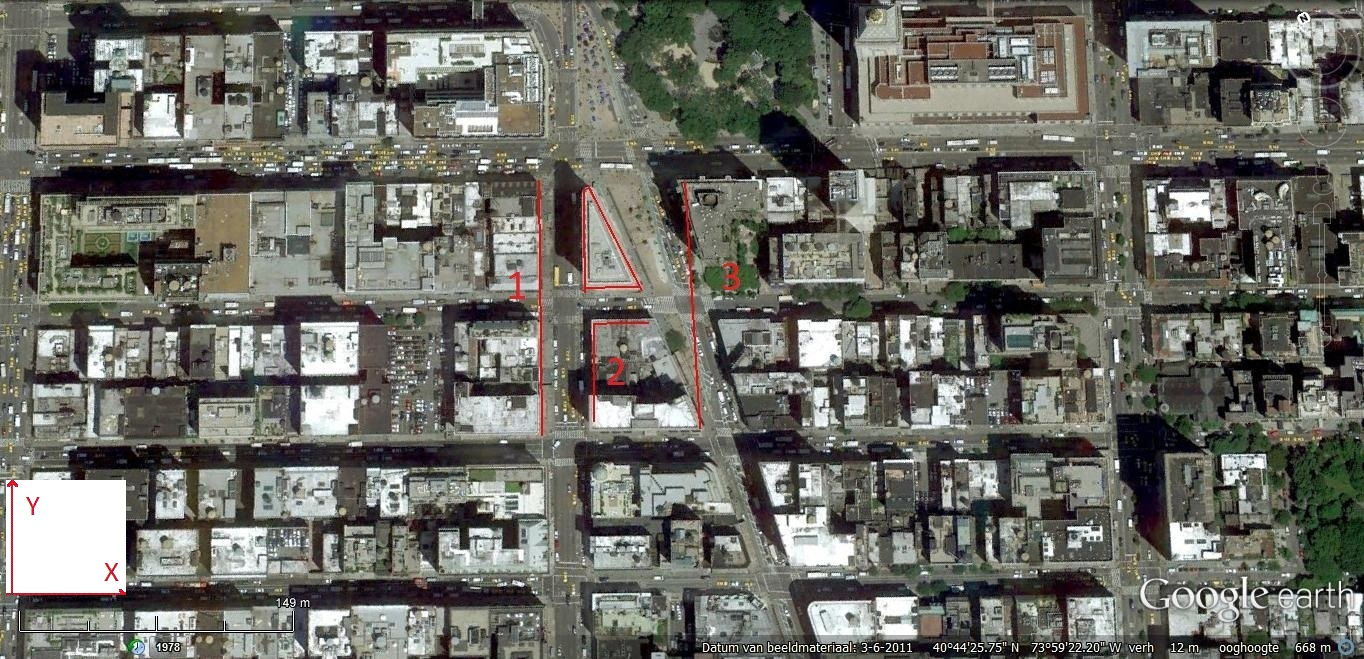
\includegraphics[width = \textwidth]{flatironafschatting.jpg}
\caption{A snapshot of the method used to estimate the dimensions using Google Maps. The red lines indicated the measured distances. }
\label{maps}
\end{figure}
From this figure and the measurement tool on the Google Maps program, we found the following dimensions for the Flatiron building and surroundings. The numbers correspond with the building numbers in table \ref{measurements}
%\begin{table}
%\centering
%\begin{tabular}
%Building No. & x-length & y-length\\
%\end{tabular}
%\end{table}
